\documentclass[tikz]{standalone}
\usepackage{fourier}
\usetikzlibrary{arrows.meta}
\usetikzlibrary{calc}
\tikzset{>=latex}
\definecolor{bookblue}{RGB}{0,173,239}
\definecolor{bookpink}{RGB}{236,0,140}
\definecolor{bookgreen}{RGB}{50,200,0}
\definecolor{bookbluearea}{RGB}{204,239,252}
\tikzstyle{blueline}=[draw=bookblue,line width=0.2mm]
\tikzstyle{pinkline}=[draw=bookpink,line width=0.2mm]
\tikzstyle{greenline}=[draw=bookgreen,line width=0.2mm]
\tikzstyle{blackline}=[draw=black,line width=0.2mm]
\tikzstyle{bluearea}=[fill=bookbluearea]

\begin{document}
  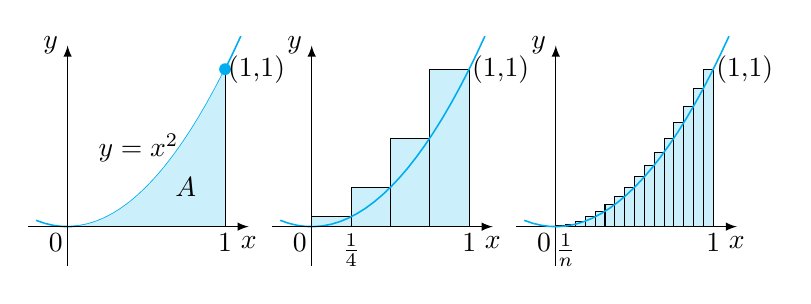
\begin{tikzpicture}
    \draw[blueline,domain=-0.4:2.2] plot (\x,{0.5*(\x)^2});
    
    \fill [bluearea,domain=-0:2,variable=\x]
    plot ({\x}, {0.5*\x*\x})
    -- (2, 0)
    -- cycle;
    %\fill[bluearea,domain=-0.4:2,variable=\x,below] plot (\x,{0.5*(\x)^2});
    \node at (1.5,0.5) {$A$};
    
    \draw (2,0) -- (2,2);
    \fill [fill=bookblue] (2,2) circle (0.075cm);
    \node at (2.4,2) {(1,1)};
    \node at (0.9,1) {$y=x^2$};
    \node at (2,-0.2) {1};
    \node at (-0.15,-0.2) {0};
    \draw[->] (-0.5,0) -- (2.3,0) node[below] {$x$};
    \draw[->] (0,-0.5) -- (0,2.3) node[left] {$y$};
    
    \begin{scope}[xshift=3.1cm]
    \draw [fill=bookbluearea] (0,0) rectangle (0.5,{0.5*0.5^2});
    \draw [fill=bookbluearea] (0.5,0) rectangle (1,{0.5*1^2});
    \draw [fill=bookbluearea] (1,0) rectangle (1.5,{0.5*1.5^2});
    \draw [fill=bookbluearea] (1.5,0) rectangle (2,{0.5*2^2});
    \draw[blueline,domain=-0.4:2.2] plot (\x,{0.5*(\x)^2});
    %\fill [fill=bookblue] (2,2) circle (0.075cm);
    \node at (2.4,2) {(1,1)};
    \node at (2,-0.2) {1};
    \node at (-0.15,-0.2) {0};
    \node at (0.5,-0.3) {$\frac{1}{4}$};
    \draw[->] (-0.5,0) -- (2.3,0) node[below] {$x$};
    \draw[->] (0,-0.5) -- (0,2.3) node[left] {$y$};
    
    \end{scope}
    
    \begin{scope}[xshift=6.2cm]
    \foreach \i in {1,...,16}{
      \draw [fill=bookbluearea] ({(\i-1)*0.125},0) rectangle (\i*0.125,{0.5*(\i*0.125)^2});
    }
    \node at (0.125,-0.3) {$\frac{1}{n}$};
    \draw[->] (-0.5,0) -- (2.3,0) node[below] {$x$};
    \draw[->] (0,-0.5) -- (0,2.3) node[left] {$y$};
    
    
    %  \draw [fill=bookbluearea] (0.125,0) rectangle (0.25,{0.5*0.25^2});
    %  \draw [fill=bookbluearea] (0.25,0) rectangle (0.375,{0.375*0.5^2});
    %  \draw [fill=bookbluearea] (0.375,0) rectangle (0.5,{0.5*0.5^2});
    %  \draw [fill=bookbluearea] (0.5,0) rectangle (0.75,{0.5*0.75^2});
    %  \draw [fill=bookbluearea] (0.75,0) rectangle (1,{0.5*1^2});
    %  \draw [fill=bookbluearea] (1,0) rectangle (1.25,{0.5*1.25^2});
    %  \draw [fill=bookbluearea] (1.25,0) rectangle (1.5,{0.5*1.5^2});
    %  \draw [fill=bookbluearea] (1.5,0) rectangle (1.75,{0.5*1.75^2});
    %  \draw [fill=bookbluearea] (1.75,0) rectangle (2,{0.5*2^2});
    \draw[blueline,domain=-0.4:2.2] plot (\x,{0.5*(\x)^2});
    %\fill [fill=bookblue] (2,2) circle (0.075cm);
    \node at (2.4,2) {(1,1)};
    \node at (2,-0.2) {1};
    \node at (-0.15,-0.2) {0};
    \end{scope}
  \end{tikzpicture}
\end{document}